\subsection{Library location}
The library is published as a \emph{Go module} to a well-known source control provider using \emph{git}. Instructions on usage, and the full source code are available on the project's home page~\cite{k-anon}. A developer intending to use the library has several options to start using it:
\begin{enumerate}
    \setstretch{1.0}
    \item add a direct dependency using Go modules \emph{(recommended)}
    \item use the \texttt{`go get'} command to download it to the \texttt{\$GOPATH}
    \item clone the source code and build it manually
\end{enumerate}

\subsection{Go modules}

\subsubsection{Adding module dependencies}

Go added support for managing direct and indirect dependencies starting from version \textit{1.11}. The implementation is based on \textit{v-go}. Direct and indirect dependencies are managed in a \texttt{go.mod} file located at the root of the project. When an import to an external module is declared in a source file, Go will automatically obtain \emph{latest} stable version of the module and it's dependencies when building the project --- this is done automatically, and normally there is no need to interact with the \texttt{go.mod} file directly. However, if needed the \texttt{`go get'} and \texttt{`go mod'} commands can be used to manage go modules explicitly (sync, upgrade, etc.).

For example, to start using the graph anonymization library with Go modules, one would add the import on Listing~\ref{lst:go_import}. Go will automatically obtain the latest stable version of the library and register the dependency in the \texttt{go.mod} file (see Listing~\ref{lst:go_mod}).

\begin{lstlisting}[caption=Importing the graph library,label=lst:go_import,float,floatplacement=H]
import "git.okki.hu/garric/k-anon"
\end{lstlisting}


\begin{lstlisting}[caption=The \texttt{go.mod} file,label=lst:go_mod,float,floatplacement=H]
require (
    github.com/gar-r/k-anon v1.2.6
    gonum.org/v1/netlib v0.0.0-20190327185612-36a5df7c87e8 // indirect
    // ...
)
\end{lstlisting}


\subsubsection{Publishing modules}

In order to \emph{publish} a Go project as a module, it needs to be under supported source control. This is usually git, but Mercurial, Bazaar and others are also supported~\cite{publish-go-modules}. Once the project repository is hosted, new releases can be created by \emph{tagging} a commit with a version using \emph{semantic versioning}. A go module's semantic version has the form of \texttt{vMAJOR.MINOR.PATH}. (Semantic versioning itself will not be discussed in this document.)

For example, for the graph anonymization library a few tagged versions can be seen on Figure~\ref{fig:tagged_versions}.
\begin{figure}[H]
    \centering
    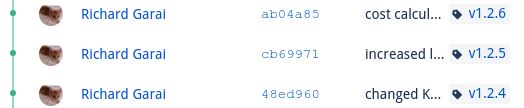
\includegraphics[width=0.8\textwidth]{tagged-versions.png}
    \caption{Tagged versions}\label{fig:tagged_versions}
\end{figure}